\subsection{离散对称性}

接下来我们来考察一些离散对称性: 空间反演, 晶格平移和时间反演.

\subsubsection{空间反演}

对于空间反演算符$\pi$, 我们要求其:

\begin{equation}
  \begin{aligned}
    \psi(x) = - (\pi \psi)(x) \mn{$(\pi \psi)(x)$是指$\psi$ 在$\pi$ 算符作用后
    得到的态在坐标表象下的波函数.}
  \end{aligned}
\end{equation}

或者对于braket记号:

\begin{equation}
  \begin{aligned}
    \bra{a}\pi^{\dagger} x \pi \ket{a} = - \bra{a}x\ket{a}
  \end{aligned}
\end{equation}

由于上式对于任意$\ket{a}$都成立, 因此可以推断出:

\begin{equation}
  \begin{aligned}
    \pi^{\dagger} x \pi = -x
  \end{aligned}
\end{equation}

而由于$\pi$ 是幺正算符, 左乘$\pi$可以得到:

\begin{equation}
  \begin{aligned}
    x \pi = - \pi x
  \end{aligned}
\end{equation}

对于坐标本征态$\ket{x}$, 其在$\pi$ 作用后变为$e^{{\rm i} \xi}\ket{-x}$:

\begin{equation}
  \begin{aligned}
    x \pi \ket{x} = - \pi x \ket{x} = -x \pi \ket{x}
  \end{aligned}
\end{equation}

即$\pi \ket{x}$ 是$x$ 的本征态, 本征值为$-x$, 因此其与$\ket{-x}$ 至多相差
一个相因子. 而由于空间反演是一个全局对称性, 因此我们总能将这个相因子取为$1$.

那么我们可以发现:

\begin{equation}
  \begin{aligned}
    \pi^{2} \ket{x} = \ket{x}
  \end{aligned}
\end{equation}

意味着$\pi^{-1} = \pi$, 同时由于$\pi$ 是幺正的, 可以得到结论$\pi$ 同时也是
厄密的, 并且本征值只能为$\pm 1$.

像位置算符 $x$ 这样满足$\pi^{\dagger} x \pi = -x$的算符被称为奇宇称算符.
类似的还有动量算符$p$. 而也存在一些像角动量算符$L$ 这样的虽然是矢量算符,
但是具有偶宇称的算符. $x,p$ 这样的算符称为矢量算符 而$L$ 称为轴矢量/赝矢量
算符.

类似的, 对于标量算符, 也可以按照其的宇称进行分类. 在空间反演作用下保持不变
的称为标量算符, 而具有奇宇称的称为赝标量.

接下来, 我们来看空间反演算符的本征态, 正如我们前面提到的, 空间反演算符的本征值
为$\pm 1$, 我们将那些本征值为$+1$ 的称为具有偶宇称的态, 而本征值为$-1$ 的称为
具有奇宇称的态. 不难看出奇偶宇称的态的波函数:

\begin{equation}
  \begin{aligned}
    \psi(x) = \bra{x}\pi \ket{a} = \pm \bra{x}\ket{a} = \bra{\pm x}\ket{a} = 
    \pm \psi(-x)
  \end{aligned}
\end{equation}

对于具有宇称的体系, 即$[\mathcal{H}, \pi] = 0$, 一定存在既是能量本征态同时也是
具有宇称的态. 但是由于简并的存在, 我们并不能断言能量本征态就是空间反演算符的
本征态. 这是由于简并的存在, 假设 $\ket{E_{n}}, \ket{E_{n}'}$ 是具有相同能量
本征值的简并态, 并且一个具有奇宇称, 一个具有偶宇称, 那么显然, 他们的线性组合
$c_1 \ket{E_{n}} + c_2 \ket{E_{n}'}$ 也是能量的本征态, 但不是空间反演算符的
本征态.

\begin{figure}[htpb]
  \centering
  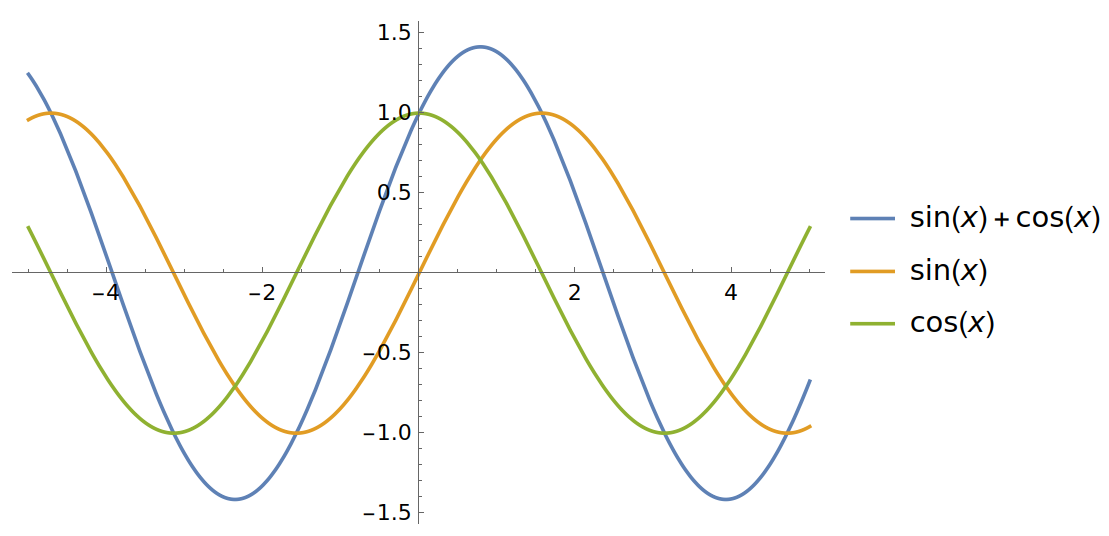
\includegraphics[width=0.8\linewidth]{figures/parity_addition_demo}
  \caption{奇宇称的$\sin x$ 和具有偶宇称的$\cos x$ 叠加出不具有宇称的态}%
  \label{fig:parity_addition_demo}
\end{figure}

因此, 只有当不存在能量简并的宇称体系, 我们才能断言任意能量本征态都是空间反演
算符的本征态.

假设有两个空间反演算符的本征态:

\begin{equation}
  \begin{aligned}
    &\pi \ket{a} = \epsilon_{a} \pi \ket{a}\\
    & \pi \ket{b} = \epsilon_{b} \pi \ket{b}
  \end{aligned}
\end{equation}

本征值$\epsilon_{a}, \epsilon_{b} = \pm 1$. 还有一个具有宇称的算符$o$ :

\begin{equation}
  \begin{aligned}
    \pi o \pi^{\dagger} = \epsilon_{o} o
  \end{aligned}
\end{equation}

那么我们有定理:

\begin{theorem}[宇称选择定则]
  除非$\epsilon_{a} \epsilon_{b} \epsilon_{o} = 1$, 否则:
  
  \begin{equation}
    \begin{aligned}
      \bra{b} o \ket{a} = 0
    \end{aligned}
  \end{equation}

\end{theorem}
\begin{proof}

  \begin{equation}
    \begin{aligned}
      \bra{b}o\ket{a} = \bra{b}\pi^{-1}\pi o \pi^{-1}\pi\ket{a} = \epsilon_{a}
      \epsilon_{b} \epsilon_{o} \bra{b} o \ket{a}
    \end{aligned}
  \end{equation}

  因此要么$\bra{b}o\ket{a} = 0$, 要么$\epsilon_{a} \epsilon_{b} \epsilon_{o}= 1$.

\end{proof}

\subsubsection{晶格平移对称性}

对于间距为$a$ 的一维晶格$V(x) = V(x\pm a)$, 定义平移算符$\tau(l)$:

\begin{equation}
  \begin{aligned}
    \tau^{\dagger}(l) x \tau(l) = x+l,\quad \tau(l) \ket{x} = \ket{x+l}
  \end{aligned}
\end{equation}

当$l = a$时, 有$[\mathcal{H}, \tau(a)] = 0$. 但是, 和空间反演变换的不同之处
在于, $\tau(a)$不是厄密的. 而我们希望得到 $\mathcal{H}$ 和$\tau(a)$ 的共同本征
态, 我们首先从晶格间势垒为无穷深的理想情况出发, 这种情况下, 不同晶格间不存在
隧穿效应, 我们取一组$\mathcal{H}$ 的本征矢 $\ket{n}$, 代表粒子局域在第 $n$ 
个晶格内. 明显, 这组本征矢是无穷维简并的, 并且不是$\tau(a)$ 的本征矢, 因为
$\tau(a) \ket{n} = \ket{n+1}$. 我们通过线性组合来构造$\mathcal{H}$ 和$\tau(a)$ 
的共同本征矢:

\begin{equation}
  \begin{aligned}
    \ket{\theta} = \sum_{n=-\infty}^{\infty} e^{{\rm i} n \theta} \ket{n}
  \end{aligned}
\end{equation}

明显, $\ket{\theta}$ 仍然是$\mathcal{H}$ 的本征态, 同时, 对于$\tau(a)$ :

\begin{equation}
  \begin{aligned}
    \tau(a) \ket{\theta} &= \sum_{n=-\infty}^{\infty} e^{{\rm i} n \theta}
    \ket{n+1} = \sum_{n=-\infty}^{\infty} e^{{\rm i} (n-1) \theta} \ket{n}\\
                         &= e^{-{\rm i} \theta} \ket{\theta}
  \end{aligned}
\end{equation} 

现在回到更现实一点的情况里来, 我们假设晶格间的能垒虽然不是无限但是足够高,
使得那些非近邻的晶格间的矩阵元可忽略, 唯一的非对角矩阵元为:

\begin{equation}
  \begin{aligned}
    \bra{n'} \mathcal{H} \ket{n} = \Delta\quad {\rm i.f.f}\; n'=n\pm 1
  \end{aligned}
\end{equation}

不难看出, $\Delta$ 是一个不依赖与$n$ 的常量. 并且现在$\ket{n}$ 不再是能量
本征态了.

但是, 这并不影响$\ket{\theta}$ 仍然是$\tau(a)$ 的本征态, 问题是, 它是$\mathcal{H}$ 
的本征态吗?

对于$\ket{n}$, 我们有:

\begin{equation}
  \begin{aligned}
    \mathcal{H} \ket{n} = E_0 \ket{n} - \Delta \ket{n+1} - \Delta \ket{n-1}
  \end{aligned}
\end{equation}

带入$\ket{\theta}$, 得到:

\begin{equation}
  \begin{aligned}
    \mathcal{H} \ket{\theta} = (E_0 - 2 \Delta \cos \theta) \ket{\theta}
  \end{aligned}
\end{equation}

可以看出, 我们解开了能量的简并, 将能量的本征值扩大到 $E_0 - 2 \Delta$ 到
$E_0 + 2 \Delta$ 之间.
